\section{Experiments}
\label{sec:experiments}

\subsection{Experimental setup}
\label{sec:experimental-setup}

\paragraph{\mbox{Models and workloads.}}
We evaluate three workloads. For supervised fine-tuning (SFT), we use
NemotronDiffusion 3B, 8B, and 14B~\citep{fu2026nemotronlabsdiffusion} and
DiffusionGemma 26B-A4B~\citep{odonoghue2026diffusiongemma}. For AR-to-BDLM
conversion, we use the text backbones of Qwen3.5-27B~\citep{qwen2026qwen35}
and Qwen3.8-27B~\citep{qwen2026qwen38} with the Fast-dLLM v2
objective~\citep{wu2025fastdllmv2}. Conversion provides a route to parallel
generation without training a diffusion model from scratch and tests CSBP
beyond fine-tuning existing BDLMs. We also train long-context DFlash2
drafters~\citep{inco2026dflash2} for Qwen3.8-27B and Muse-Glimmer-30B following
the SpecForge framework~\citep{li2026specforge} and open-source
implementation~\citep{specforge2025} (Appendix~\ref{app:dflash2-objective}).
Across all workloads, the best baseline and CSBP evaluate the same objective on the same
target blocks. The SFT and AR-to-BDLM workloads include every eligible target
block, while DFlash2 uses the draft blocks sampled by its training objective.

\paragraph{\mbox{Hardware.}}
Full-model training uses two nodes, each with eight NVIDIA H200 GPUs and
141\,GB of HBM3e per GPU. DFlash2 training uses one node with eight NVIDIA
H100 GPUs and 80\,GB of HBM3 per GPU.

\paragraph{\mbox{Baselines and configurations.}}
We compare against highly optimized conventional training without BP, using
the token-position sharding found in distributed-training
libraries~\citep{nvidia_megatron_cp,pytorch_torchtitan} when CP is required. We
profile-optimize baseline execution and share applicable kernel and layout
optimizations with CSBP. For each setting, the best baseline is the
highest-throughput tested feasible combination of data,
tensor~\citep{shoeybi2019megatron}, expert~\citep{lepikhin2020gshard},
context~\citep{liu2023ringattention,jacobs2023ulysses}, and sequence
parallelism~\citep{korthikanti2022recomputation} and global batch size. With
CSBP, each complete corrupted-block computation stays on one rank while the
reusable clean context remains sharded across ranks, eliminating cross-rank
transport of corrupted K/V and their gradients. We optimize topology and batch
size independently with CSBP enabled.

\paragraph{\mbox{Implementation and metrics.}}
We use PyTorch~\citep{paszke2019pytorch},
FlashAttention-4~\citep{zadouri2026flashattention4},
FlexAttention~\citep{dong2025flexattention}, and NCCL; all runs use BF16.
We implement a token-chunked linear cross-entropy loss with cuBLAS
projections and fused CUDA softmax/CE kernels, avoiding full-sequence logits
materialization.
Full-model runs use activation checkpointing~\citep{chen2016checkpointing} and
DeepSpeed ZeRO Stage~2~\citep{rajbhandari2019zero}; the
throughput-maximizing DFlash2 recipe uses fused AdamW without activation
checkpointing. We report useful model FLOPs utilization
(MFU)~\citep{chowdhery2022palm}. For DFlash2, throughput and useful MFU count
supervised draft-target tokens; computation replicated across context ranks
consumes runtime without increasing either metric. Peak HBM is the maximum
peak allocated memory across GPUs. For throughput and memory profiles, every training sequence has
exactly the reported context length. The equal-wall-clock experiments use the
variable sequence lengths of their respective datasets.

\subsection{Effectiveness of CSBP}
\label{sec:main-256k-results}

CSBP improves throughput across every evaluated model and both training
objectives at 256K context (Table~\ref{tab:main-256k-results}). It delivers
$1.18$--$1.45\times$ speedup for SFT and $1.27$--$1.33\times$ for AR-to-BDLM conversion, while matching or reducing peak HBM. The gains extend from
NemotronDiffusion to DiffusionGemma 26B-A4B and both Qwen backbones, demonstrating consistent
benefits across the evaluated model families.

% The SFT rows exactly reuse the selected 256K measurements in
% tables/two_node_h200_1p2_results.tex. The AR-to-BDLM rows exactly reuse the
% 256K measurements in tables/appendix_fast_dllm_v2_scaling.tex.
\begin{table}[!htb]
  \centering
  \caption{CSBP accelerates training at 256K context.}
  \label{tab:main-256k-results}
  \small
  \setlength{\tabcolsep}{4pt}
  \renewcommand{\arraystretch}{1.35}
  \resizebox{\linewidth}{!}{%
  \begin{tabular}{@{}llllrrrr@{}}
    \toprule
    \shortstack{Training\\workload} & Model & \shortstack{Best baseline\\topology} & \shortstack{Ours\\topology} & Tok/s & Speedup & \shortstack{MFU\\(\%)} & \shortstack{Peak HBM\\(GiB)} \\
    \midrule
    BDLM fine-tuning & NemotronDiffusion 3B & DP4/TP1/CP4 & DP4/TP1/CP4/BP4 & 13{,}434 / \textbf{16{,}027} & \textbf{1.19$\times$} & 31.7 / \textbf{37.8} & 57.1 / \textbf{57.0} \\
    BDLM fine-tuning & NemotronDiffusion 8B & DP4/TP1/CP4 & DP4/TP1/CP4/BP4 & 9{,}668 / \textbf{11{,}379} & \textbf{1.18$\times$} & 32.3 / \textbf{38.0} & 97.5 / 97.5 \\
    BDLM fine-tuning & NemotronDiffusion 14B & DP2/TP1/CP8 & DP2/TP1/CP8/BP8 & 7{,}884 / \textbf{9{,}301} & \textbf{1.18$\times$} & 33.1 / \textbf{39.0} & 91.1 / \textbf{90.6} \\
    BDLM fine-tuning & DiffusionGemma 26B-A4B & DP1/TP1/EP2/CP8 & DP1/TP1/EP2/CP8/BP8 & 10{,}557 / \textbf{15{,}359} & \textbf{1.45$\times$} & 12.7 / \textbf{18.4} & 118.1 / \textbf{113.6} \\
    \midrule
    AR-to-BDLM conversion & Qwen3.8-27B & DP1/TP2/CP8 & DP1/TP2/CP8/BP8 & 2{,}623 / \textbf{3{,}490} &
    \textbf{1.33$\times$} & 20.1 / \textbf{26.8} & 120.7 / \textbf{111.1} \\
    AR-to-BDLM conversion & Qwen3.5-27B & DP1/TP2/CP8 & DP1/TP2/CP8/BP8 & 2{,}641 / \textbf{3{,}351} &
    \textbf{1.27$\times$} & 20.3 / \textbf{25.7} & 120.7 / \textbf{111.1} \\
    \bottomrule
  \end{tabular}}
  \par\vspace{2pt}
  \parbox{\linewidth}{\footnotesize\raggedright Pairs: best baseline~/~ours. Bold marks the better value.}
\end{table}


\subsection{Scaling with CP/BP degree}
\label{sec:parallel-degree-scaling}

CSBP's advantage grows as training uses more ranks to accommodate longer
contexts (Figure~\ref{fig:parallel-degree-scaling}). From degree two to eight,
speedup rises from $1.10\times$ to $1.18\times$ for NemotronDiffusion 14B and from
$1.25\times$ to $1.45\times$ for DiffusionGemma 26B-A4B.
Keeping corrupted-block computation local becomes increasingly beneficial
in this long-context regime.

\begin{figure}[!htb]
  \centering
  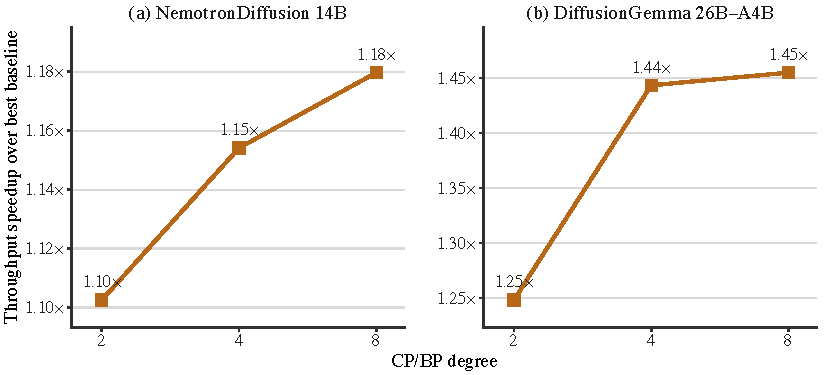
\includegraphics[width=0.92\linewidth]{figures/parallel_degree_scaling.pdf}
  \caption{CSBP's throughput gains grow with CP/BP degree.}
  \label{fig:parallel-degree-scaling}
\end{figure}

\subsection{Scaling with context length}
\label{sec:sequence-length-scaling}

Longer contexts strengthen the throughput advantage of CSBP
(Figure~\ref{fig:sequence-length-scaling}). Extending context from 64K to 512K
increases speedup from $1.10\times$ to $1.19\times$ for NemotronDiffusion 14B and from
$1.25\times$ to $1.61\times$ for DiffusionGemma 26B-A4B. The gains persist through
512K, consistent with avoiding corrupted K/V communication becoming more
valuable as sequences grow.

\begin{figure}[!htb]
  \centering
  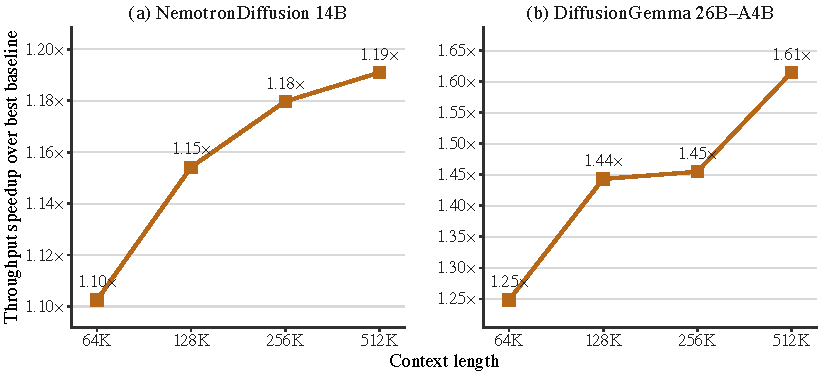
\includegraphics[width=0.8\linewidth]{figures/sequence_length_scaling.pdf}
  \caption{Longer contexts amplify CSBP's throughput advantage.}
  \label{fig:sequence-length-scaling}
\end{figure}

Context sharding is what makes these long-context gains practical.
Without it, BP replicates overlapping clean prefixes: NemotronDiffusion 14B pure BP
is slower and uses more memory at 64K, then runs out of memory at 128K;
DiffusionGemma 26B-A4B pure BP runs out of memory at both 64K and 128K under
the matched native objective.
CSBP fits and accelerates training in these cases
(Appendix~\ref{app:pure-bp-ablation}).

\subsection{Accelerating block diffusion speculative decoding drafter training}
\label{sec:dflash2-scaling}

On eight H100 GPUs (Table~\ref{tab:dflash2-h100-scaling}), CSBP produces larger
DFlash2 speedups than full-model workloads because conventional CP replicates
the block-local decoder, vocabulary loss, and selector across context ranks,
whereas CSBP assigns each draft block to one rank. At 512K, removing this two-way duplication
yields $2.48\times$ higher throughput; at 1M, four CP2/BP2 replicas versus one
CP8 baseline yield $7.59\times$. Executed-GEMM utilization (executed GEMM
FLOP/s relative to BF16 peak) is 28.7\%/37.0\% at 512K and 35.8\%/36.5\% at 1M
for baseline/CSBP. At 512K, CSBP cuts exposed attention communication from
105.4 to 7.5\,ms per GPU because each block stays on one rank, avoiding
corrupted K/V and gradient transport and explaining its higher utilization;
the near-equal 1M values show the gains reflect genuine reductions in executed
work and increased data parallelism. At 256K, where full replicas fit, DP8 remains
19.2\% faster because it avoids sequence-parallel overhead.

Muse-Glimmer-30B shows complementary gains. Against the fastest
feasible non-BP topology, CSBP is $1.56\times$, $3.35\times$, and $4.81\times$
faster at 256K, 512K, and 1M, respectively. At 512K, CP2 runs out of memory,
while CP2/BP2 fits and supports four data-parallel replicas; at 1M, CP4/BP4
both saves 12.0\% peak HBM relative to CP8 and raises throughput by
$4.81\times$.

% Single-node DFlash2 run provenance (8x H100 80 GB, four warmups and four
% measured complete optimizer steps):
% 256K best baseline, DP8:
% /persistent/runs/qwen3.8_27b_dflash2_262144_h100_dflash_20260912_230144
% 256K ours, DP4/CP2/BP2:
% /persistent/runs/qwen3.8_27b_dflash2_262144_h100_dflash_20260912_203541
% 512K pair, DP4/CP2 and DP4/CP2/BP2:
% /persistent/runs/qwen3.8_27b_dflash2_524288_h100_dflash_20260912_212734
% 1M best baseline, DP1/CP8:
% /persistent/runs/qwen3.8_27b_dflash2_1048576_h100_dflash_20260912_230426
% 1M ours, DP4/CP2/BP2:
% /persistent/runs/qwen3.8_27b_dflash2_1048576_h100_dflash_20260912_213533
% Muse-Glimmer-30B final topology matrices:
% 256K: /persistent/runs/muse_glimmer_30b_dflash2_262144_h100_dflash_20260916_094323
% 512K: /persistent/runs/muse_glimmer_30b_dflash2_524288_h100_dflash_20260916_094634
% 1M: /persistent/runs/muse_glimmer_30b_dflash2_1048576_h100_dflash_20260916_092643
\begin{table}[!htb]
  \centering
  \caption{CSBP accelerates long-context DFlash2 drafter training.}
  \label{tab:dflash2-h100-scaling}
  \small
  \setlength{\tabcolsep}{4pt}
  \renewcommand{\arraystretch}{1.35}
  \resizebox{\linewidth}{!}{%
  \begin{tabular}{@{}llllrrrr@{}}
    \toprule
    Model & \shortstack{Context\\length} & \shortstack{Best baseline\\topology} & \shortstack{Ours\\topology} & Tok/s & Speedup & \shortstack{MFU\\(\%)} & \shortstack{Peak HBM\\(GiB)} \\
    \midrule
    Qwen3.8-27B & 256K & DP8 & DP4/CP2/BP2
      & \textbf{167{,}228} / 140{,}350 & 0.84$\times$
      & \textbf{38.4} / 32.2
      & 63.5 / \textbf{48.3} \\
    Qwen3.8-27B & 512K & DP4/CP2 & DP4/CP2/BP2
      & 57{,}027 / \textbf{141{,}222} & \textbf{2.48$\times$}
      & 13.1 / \textbf{32.4}
      & 63.3 / \textbf{54.6} \\
    Qwen3.8-27B & 1M & DP1/CP8 & DP4/CP2/BP2
      & 18{,}389 / \textbf{139{,}541} & \textbf{7.59$\times$}
      & 4.2 / \textbf{32.0}
      & \textbf{53.7} / 67.1 \\
    \midrule
    Muse-Glimmer-30B & 256K & DP4/CP2 & DP4/CP2/BP2
      & 62{,}698 / \textbf{98{,}046} & \textbf{1.56$\times$}
      & 18.5 / \textbf{28.9}
      & 63.8 / \textbf{57.5} \\
    Muse-Glimmer-30B & 512K & DP2/CP4 & DP4/CP2/BP2
      & 29{,}493 / \textbf{98{,}785} & \textbf{3.35$\times$}
      & 8.7 / \textbf{29.1}
      & \textbf{63.8} / 65.6 \\
    Muse-Glimmer-30B & 1M & DP1/CP8 & DP2/CP4/BP4
      & 12{,}842 / \textbf{61{,}742} & \textbf{4.81$\times$}
      & 3.8 / \textbf{18.2}
      & 63.3 / \textbf{55.7} \\
    \bottomrule
  \end{tabular}}
  \par\vspace{2pt}
  \parbox{\linewidth}{\footnotesize\raggedright Pairs: best baseline~/~ours. Tok/s and MFU count supervised draft-target tokens. Bold marks the better value.}
\end{table}


\subsection{Equal-wall-clock downstream performance}
\label{sec:equal-wall-clock}

We finally test whether CSBP's higher training throughput translates into
faster downstream progress under a fixed wall-clock budget. We fine-tune
DiffusionGemma 26B-A4B with the best baseline and CSBP for 12 hours and
evaluate checkpoints every three hours on SWE-bench Verified and Terminal-Bench Lite
(Figure~\ref{fig:equal-wall-clock-downstream}). We train with LoRA adapters on
eight H100 GPUs, comparing CP8 with CSBP at CP8/BP8. Appendix~\ref{app:training-evaluation-details}
provides full data and training details. CSBP achieves a higher pass
rate at every trained checkpoint on both benchmarks. Its lead peaks at 1.8
percentage points on SWE-bench Verified and 2 points on Terminal-Bench Lite;
after 12 hours, it remains 1 point ahead on both benchmarks.

\begin{figure}[!htb]
  \centering
  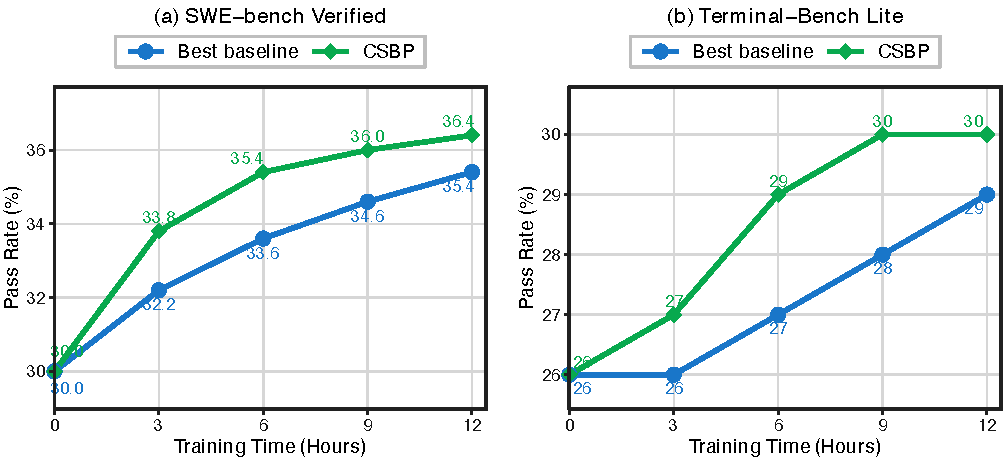
\includegraphics[width=0.95\linewidth]{figures/equal_wall_clock_downstream.pdf}
  \caption{Equal-wall-clock downstream performance. Checkpoints from the
  best baseline and CSBP are evaluated every three hours on
  (a) SWE-bench Verified and
  (b) Terminal-Bench Lite.}
  \label{fig:equal-wall-clock-downstream}
\end{figure}
